\documentclass[12pt,a4paper]{article}%
%Options -- Point size:  10pt (default), 11pt, 12pt
%        -- Paper size:  letterpaper (default), a4paper, a5paper, b5paper
%                        legalpaper, executivepaper
%        -- Orientation  (portrait is the default)
%                        landscape
%        -- Print size:  oneside (default), twoside
%        -- Quality      final(default), draft
%        -- Title page   notitlepage, titlepage(default)
%        -- Columns      onecolumn(default), twocolumn
%        -- Equation numbering (equation numbers on the right is the default)
%                        leqno
%        -- Displayed equations (centered is the default)
%                        fleqn (equations start at the same distance from the right side)
%        -- Open bibliography style (closed is the default)
%                        openbib
% For instance the command
%           \documentclass[a4paper,12pt,leqno]{article}
% ensures that the paper size is a4, the fonts are typeset at the size 12p
% and the equation numbers are on the left side
%====================Tabelas==============================================
\usepackage{multirow}
%=============================Símbolos Matemáticos=====================================================================
\usepackage{amsmath}
\usepackage{amsfonts}
\usepackage{amssymb}
%=======================================Figuras===========================================================
\usepackage{graphicx}
%\usepackage{wrapfig}
\usepackage{float}
\usepackage{tikz}
%=====================================Língua e acentos=============================================================
\usepackage[brazil]{babel}
\usepackage[utf8]{inputenc}
\usepackage[T1]{fontenc}
%========================================Espaçamento==========================================================
\usepackage[top=3cm, bottom=2cm, left=2cm, right=2cm]{geometry}
\usepackage{indentfirst}
%=======================================Lista de códigos===========================================================
\usepackage{listings}                   % para formatar código-fonte
\lstset{numbers=left, numberstyle=\tiny, stepnumber=1, numbersep=5pt, basicstyle=\scriptsize , frame=trbl}
%======================================Latexdraw============================================================
%\usepackage[usenames,dvipsnames]{pstricks}
%\usepackage{epsfig}
%\usepackage{pst-grad} % For gradients
%\usepackage{pst-plot} % For axes
%==================================================================================================
%-------------------------------------------

\begin{document}

\begin{titlepage}
\begin{center}
\begin{figure}[h]

\includegraphics[scale=0.76]{Imagens/topdotitulo.png}
\end{figure}
\rule{\columnwidth}{1.5mm}
\

\large David Maykon Krepsky Silva\\
\large Havena Louise Pavão

\vspace{4cm}
{\bf \Large Título do Experimento}
\vspace{3.5cm}

\begin{flushright}
Data de realização do experimento:\\
XX de abril de 2016\\
Série/Turma:\\
1000/1011\\
Prof. Me. Jaime Laelson Jacob 
\end{flushright}

\vspace{3.2cm}
\today

\rule{\columnwidth}{1.3mm}
\end{center}
\end{titlepage}

\section{Resumo}
Análise prática de circuitos Moduladores e Demoduladores Digitais FSK.
\newpage
\newpage

\tableofcontents

\newpage
\section{Introdução}
Dada a sua vasta aplicação em sistemas de telecomunicações, as técnicas de modulação e demodulação FSK são conhecimentos fundamentais para o engenheiro eletricista. É encontrada em vários cenários, indo desde a transmissão de sinais sem fio, até a comunicação em linhas de transmissão de potência.
Neste trabalho foi abordado, de forma experimental, a análise do funcionamento de um esquema de comunicação FSK (\textit{Frequency Shift Keying}), onde foram utilizados um circuito modulador com VCO e um demodulador não-coerente, onde o objetivo principal é proporcionar ao aluno um melhor entendimento das condições de operação dos tais circuitos eletrônicos.

\newpage
\section{Teoria}

\section{Modulação BFSK}
A modulação FSK ("\emph{Frequency Shift Keying}") é uma técnica de modulação que consiste em variar a frequência da portadora em função do sinal modulante, no caso o sinal digital a ser transmitido.
Pode-se considerar que este tipo de modulação é equivalente a modulação FM analógica.

A amplitude da onda portadora modulada é mantida constante durante todo o processo de modulação, quando o sinal digital apresenta nível lógico "1" a frequência da portadora é alterada para posteriormente ser detectada no processo de demodulação.
A frequência resultante transmitida será a frequência da onda portadora $f_c$ diminuida de uma frequência de desvio $f_d$.
Ou seja
\begin{equation}
    f_r = f_c - f_d
\end{equation}

Para a ocorrência de um nível lógico "0", a frequência resultante será a frequência da portadora mais a frequência de desvio.
\begin{equation}
    f_r = f_c + f_d
\end{equation}

\begin{figure}[H]
    \centering
    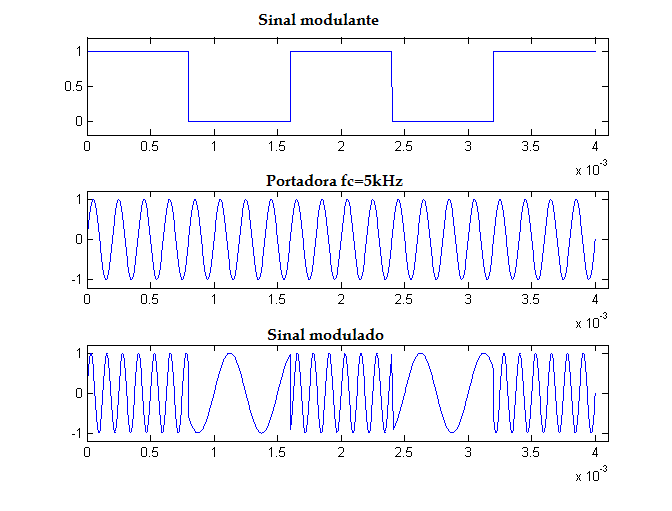
\includegraphics[scale=0.9]{imagem/fsk.png}
    \caption{Modulação FSK}
    \label{fig:mdfsk}
\end{figure}

 A Figura \ref{fig:mdfsk} mostra um sinal modulante, uma portadora $f_c=5kHz$ com $f_d = 3kHz$.
 É possível observar um sinal em $8kHz$ quando o sinal modulante é "1" e em $2kHz$ quando o sinal modulante é "0", ou seja, o esquema FSK se utiliza da frequência como um meio de transportar a informação, sendo que, para cada frequência $f_i$, é mapeado um simbolo $s_i$.
 
A largura de banda utilizada na transmissão de sinais modulados em FSK é:
\[
    BW = 2\cdot \Delta f +2B.
\]

Onde $BW$ é a largura de banda ocupada, $\Delta f$ é a variação de frequência para representar os bits e $B$ é a banda ocupada desde  $f_c + \Delta f$ até o primeiro nódulo da onda \textit{sinc}, a qual representa o espectro de um nível do sinal. 
Esse fato fica evidente ao analisarmos a figura \ref{fig:bw}, a qual mostra o espectro de um sinal FSK.

\begin{figure}[H]
    \centering
    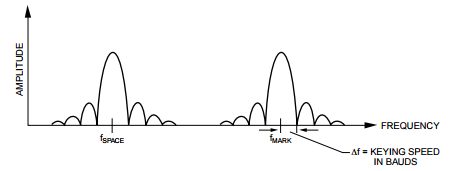
\includegraphics[scale=0.9]{imagem/bw}
    \caption{Espectro de uma sinal modulado com FSK.}
    \label{fig:bw}
\end{figure}

\section{Circuito modulador FSK}

A figura \ref{fig:modulador} representa o diagrama de blocos de um modulador FSK, onde um sinal de mensagem entra em \textit{Digital Signal} e, através do VCO (\textit{Voltage Controled Oscillator}), modifica a frequência da onda de saída. A frequência da portadora, $f_c$, é dada por um circuito que pode ser feito com um resistor e um capacitor, os quais determinam o período de oscilação da frequência central.

\begin{figure}[H]
    \centering
    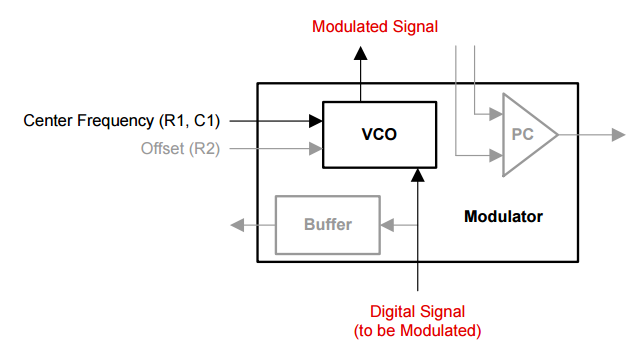
\includegraphics[scale=0.5]{imagem/modulador}
    \caption{Modulador FSK com VCO.}
    \label{fig:modulador}
\end{figure}
\section{Circuito demodulador}

O detector utilizado é um detector coerente, ou seja, possui as informações de fase e frequência da portadora. O método escolhido para a demodulação é através de um PLL, o qual rastreia a frequência do sinal recebido de forma a ser aplicada no detector coerente.



\begin{figure}[H]
    \centering
    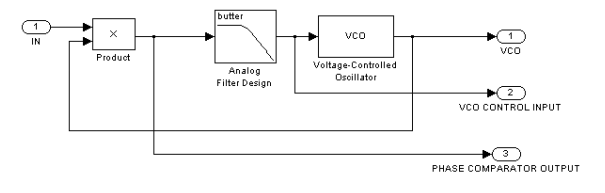
\includegraphics[scale=0.5]{imagem/coerente}
    \caption{Detector coerente com PLL.}
    \label{fig:detector}
\end{figure}

O funcionamento do circuito da figura \ref{fig:circuito} é melhor entendido se analisarmos o diagrama de blocos da figura \ref{fig:detector}. Nesta imagem é possível ver que o trabalho do CI 565 consiste em extrair as informações de fase e frequência do sinal transmito, de modo a produzir, com um VCO, um sinal semelhante, o qual é utilizado como referência para aplicação no detector coerente.

Desta forma é possível obter na saída a representação binaria do dado transmitido.

\newpage


\section{Metodologia e Desenvolvimento}

\subsection{Modulador FSK}

A partir do gerador de áudio do módulo MCA 8801, foi gerado uma onda quadrada, simulando dessa forma um trem de pulsos, do tipo NRZ (Non-Return-to-Zero). O sinal foi ajustado para uma frequência de $1 kHz$, tensão de $400 mV_p$ e ciclo ativo de $50 \%$.

Para ajusta a portadora do modulador FSK contido no módulo MCA 8801, foi ajustado, sem sinal de dados, uma frequência de $10 kHz$ a uma tensão de $1 V_p$. 

Ajustado o sinal de dados e a portadora, os sinal de dados foi ligado no modulador, podendo assim obter os respectivos sinais mostrados na figura \ref{fig:00}


\begin{figure}[H]
\centering
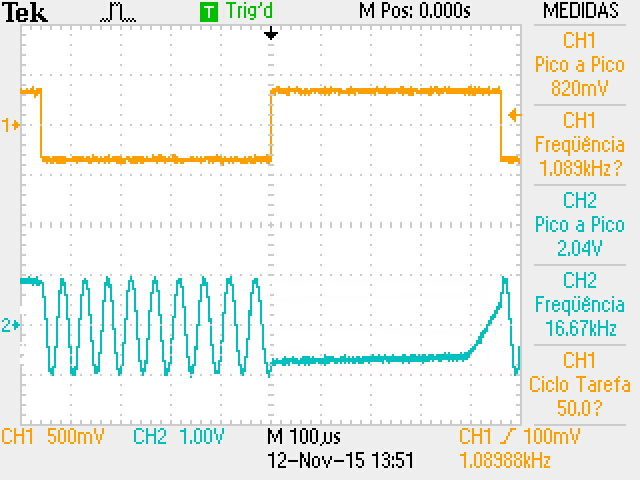
\includegraphics[scale=0.5]{imagem/TEK0000}
\caption{Sinal Modulante e Modulado.}
\label{fig:00}
\end{figure}

De forma a obter o deslocamento de frequência em resposta a onda quadrada, foi-se variando a amplitude do sinal de dados e, utilizando o cursor do osciloscópio, para obter as frequências $f_1$ e $f_2$. Os resultados foram montados na seguinte tabela.

 
\begin{table}[H]
\centering
\begin{tabular}{|l|l|l|l|}
\hline
$V_p [mV]$ & $f_1 [kHz]$  & $f_2 [kHz]$ & $2 \Delta{f} [kHz]$ \\ 
\hline
400 & 19,10 & - & - \\ 
\hline
360 & 19,23 & - & - \\ 
\hline
320 & 20,83 & - & - \\ 
\hline
280 & 16,13 & 3,67 & 12,46 \\ 
\hline
240 & 16,67 & 4,63 & 12,04 \\ 
\hline
200 & 14,71 & 4,71 & 10,00 \\ 
\hline
160 & 13,89 & 6,58 & 7,31 \\ 
\hline
120 & 13,16 & 7,82 & 5,34 \\ 
\hline
80 & 11,36 & 9,26 & 2,10 \\ 
\hline
40 & 11,36 & 10,00 & 1,36 \\ 
\hline
\end{tabular}
\end{table}

\begin{figure}[H]
\centering
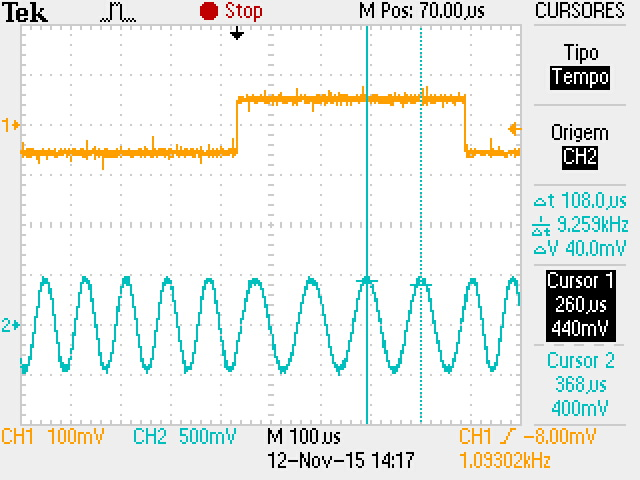
\includegraphics[scale=0.5]{imagem/TEK0005}
\caption{Obtenção de $f_2$ para $80 mV_p$.}
\label{fig:05}
\end{figure}

\begin{figure}[H]
\centering
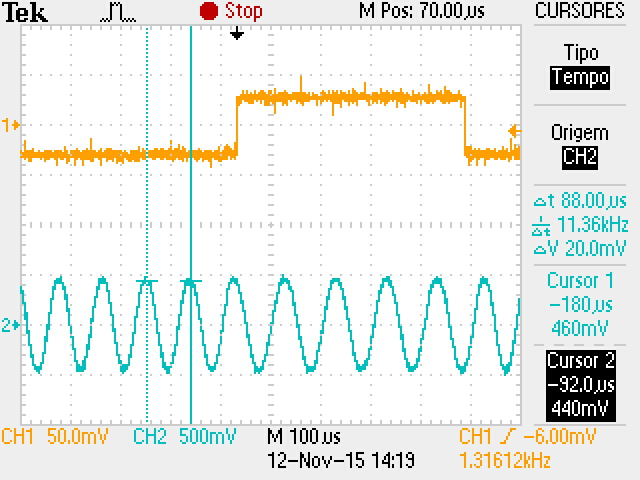
\includegraphics[scale=0.5]{imagem/TEK0006}
\caption{Obtenção de $f_1$ para $80 mV_p$.}
\label{fig:06}
\end{figure}

\begin{figure}[H]
\centering
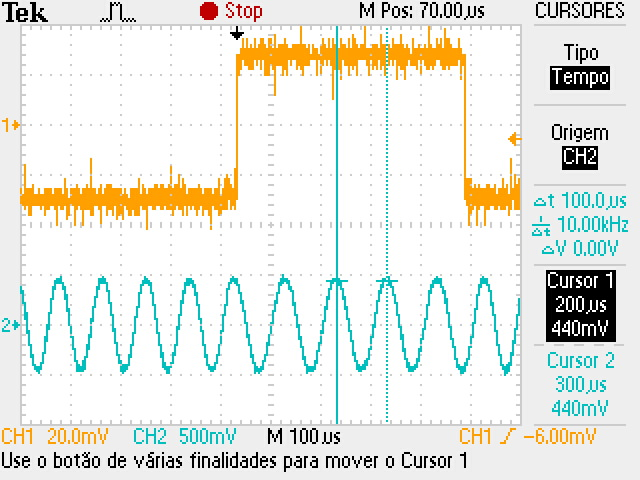
\includegraphics[scale=0.5]{imagem/TEK0007}
\caption{Obtenção de $f_2$ para $40 mV_p$.}
\label{fig:07}
\end{figure}

\begin{figure}[H]
\centering
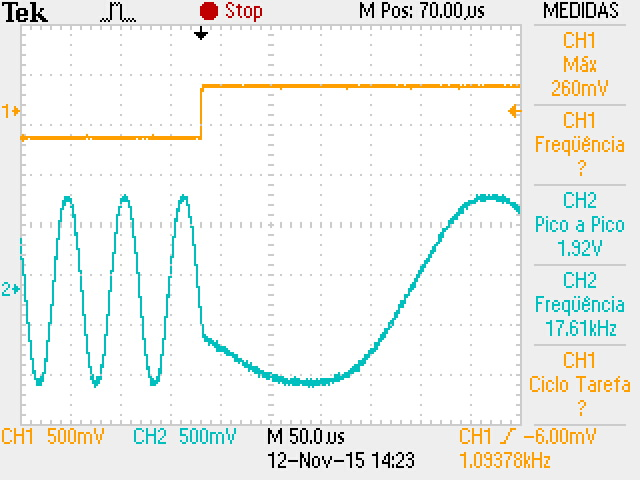
\includegraphics[scale=0.5]{imagem/TEK0008}
\caption{Obtenção de $f_1$ para $40 mV_p$.}
\label{fig:08}
\end{figure}


Observe na tabela, que somente existirá valor mensurável de $f_2$ quando $V_p \geq 280 mV$. Isso indica que o sinal só será FSK quando sua tensão de pico assumir valores menores que $280 mV$, caso contrário, é muito difícil verificar a forma de onda quando há um bit ‘1’, conforme as figuras \ref{fig:01} e \ref{fig:02}.

\begin{figure}[H]
\centering
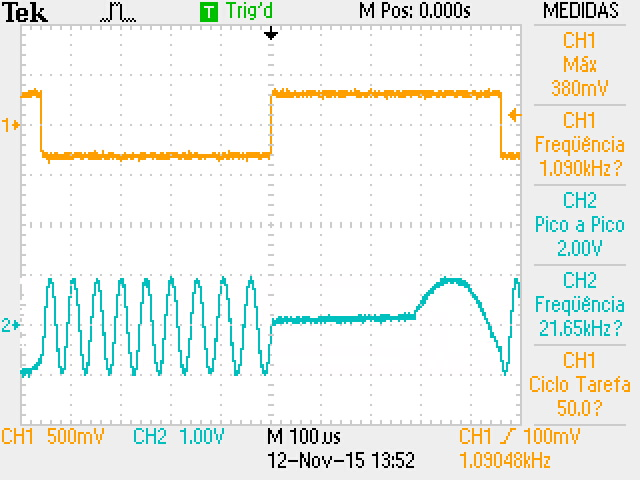
\includegraphics[scale=0.5]{imagem/TEK0001}
\caption{Sinal Modulante e Modulado para $380 mV_p$.}
\label{fig:01}
\end{figure}

\begin{figure}[H]
\centering
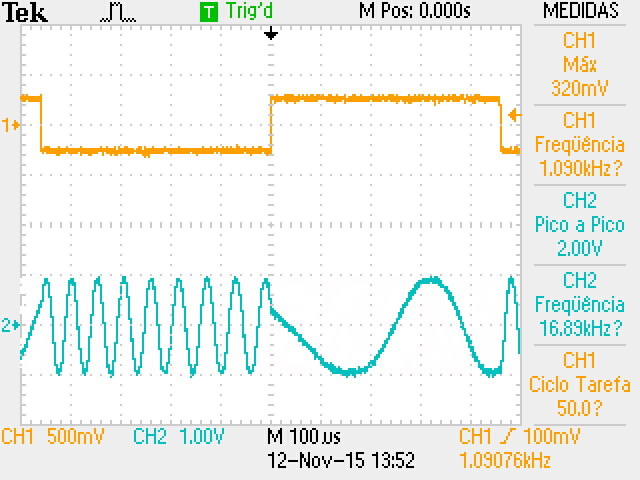
\includegraphics[scale=0.5]{imagem/TEK0002}
\caption{Sinal Modulante e Modulado para $320 mV_p$.}
\label{fig:02}
\end{figure}

Na figura \ref{fig:03} mostra o limiar de funcionamento do FSK, observe que a forma de onda quando ocorre bit ‘1’ é bem definida.

\begin{figure}[H]
\centering
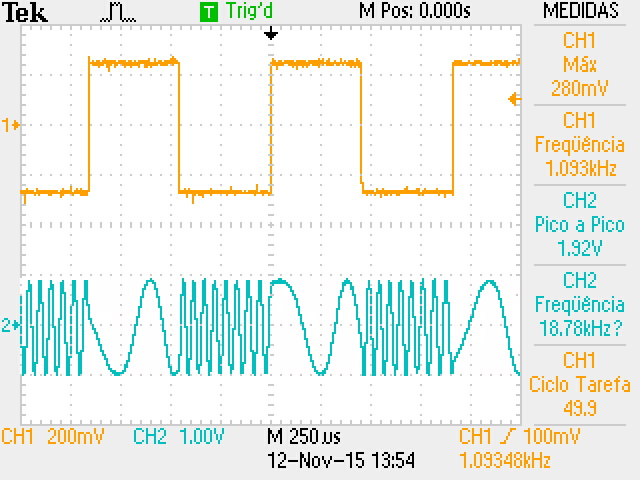
\includegraphics[scale=0.5]{imagem/TEK0003}
\caption{Sinal Modulante e Modulado para $280 mV_p$.}
\label{fig:03}
\end{figure}



De modo a determinar se existe linearidade entre tensão modulante e frequência modulada, foi gerada através do Matlab, uma curva relacionando $V_p$ x $2 \Delta{f}$.

\begin{figure}[H]
\centering
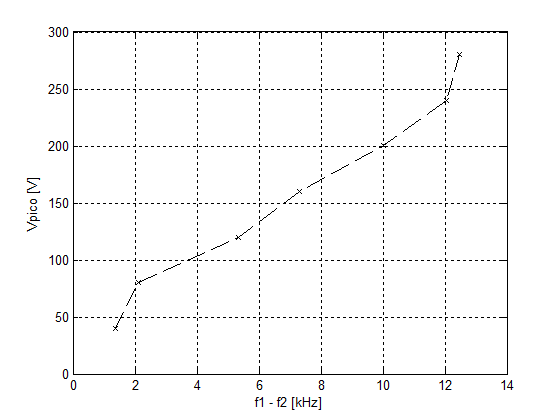
\includegraphics[scale=0.8]{imagem/curva.png}
\caption{ $V_p$ x $2 \Delta{f}$.}
\label{fig:curva}
\end{figure}

Embora, a curva não seja puramente linear, podemos dizer que a relação é linear uma vez que devemos levar em consideração possíveis imprecisões e erros de medição e calibração. Mesmo assim, o resultado é bastante consistente. 

Na figura \ref{fig:08} vemos uma descontinuidade de fase. Isso ocorre quando $2 \Delta{f}$ não é múltiplo da taxa de bit ($\frac{1}{T_b}$).


\begin{figure}[H]
\centering
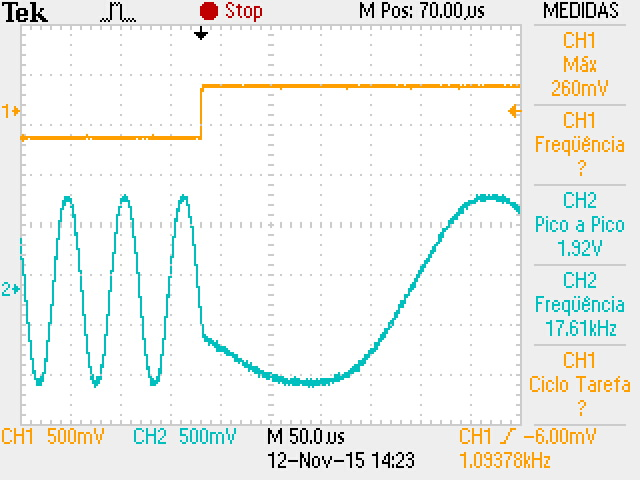
\includegraphics[scale=0.5]{imagem/TEK0008}
\caption{Descontinuidade de Fase do FSK.}
\label{fig:08}
\end{figure}


\subsection{Demodulador}

Para a demodulação do sinal modulado FSK, foi montado o circuito da figura \ref{fig:circuito}, com base no CI 565 que corresponde a um PLL (Phase-Locked Loop).

\begin{figure}[H]
\centering
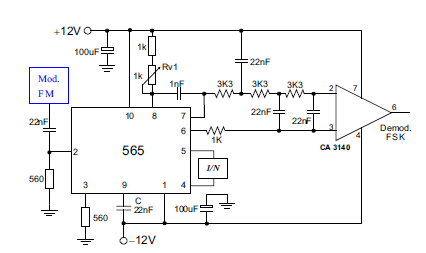
\includegraphics{imagem/circuito.png}
\caption{Circuito Demodulador FSK.}
\label{fig:circuito}
\end{figure}

Conectado o modulador e com um ajuste fino em $R_{v1}$, foi possível recuperar o sinal modulante conforme a figura \ref{fig:09}.

\begin{figure}[H]
\centering
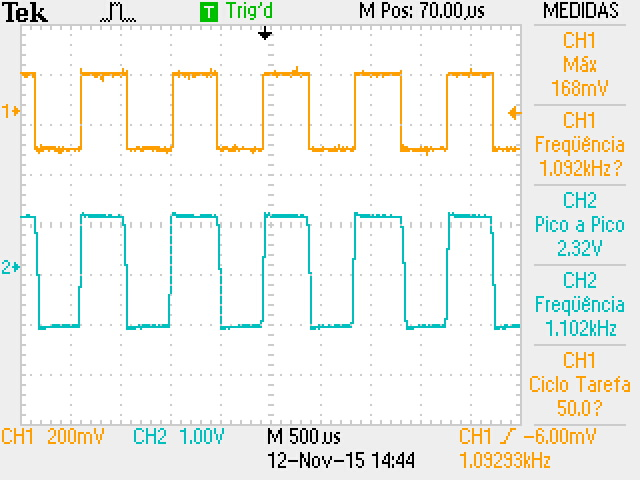
\includegraphics[scale=0.5]{imagem/TEK0009}
\caption{Sinal Modulante e Sinal Demodulado.}
\label{fig:09}
\end{figure}

Ao desconectar a entrada de dados do modulador e posteriormente, conectar a entrada do modulador ao ground, foi realizada a medição da frequência correspondente a saída VCO (pino 4). Dessa forma, encontramos uma frequência VCO de $10,66 kHz$.

\begin{figure}[H]
\centering
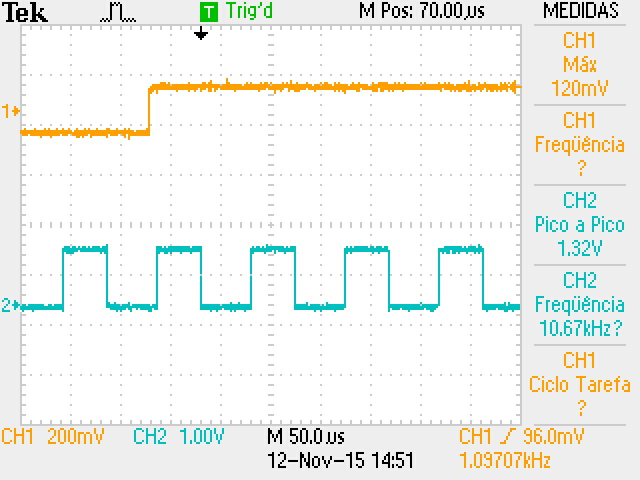
\includegraphics[scale=0.5]{imagem/TEK0010}
\caption{Frequência VCO sem dados.}
\label{fig:10}
\end{figure}

Reconectando a entrada de dados no modulador, podemos também verificar a frequência correspondente a saída VCO. Sendo assim, encontramos agora uma frequência de $13,18 kHz$.

\begin{figure}[H]
\centering
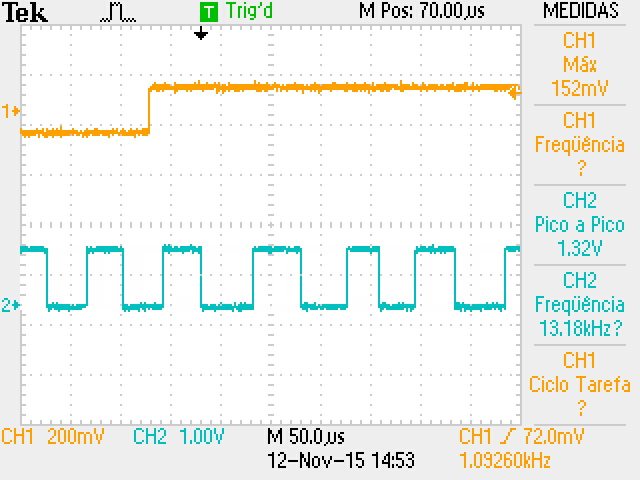
\includegraphics[scale=0.5]{imagem/TEK0011}
\caption{Frequência VCO com dados.}
\label{fig:11}
\end{figure}

\newpage
\section{Conclusão}
O presente experimento teve como objetivo verificar a modulação FSK através do módulo MCA 8801 e a demodulação FSK com base no CI 565 PLL.
Para modulação observou-se que só é possível estimar $f_2$ para sinal modulante com $V_p\leq280mV$, caso contrário é díficil identificar quando há um bit "1" no sinal modulante.
Verificou-se também que existe uma relação linear entre a tensão modulante e a frequência modulada.

Com o circuito de demodulação foi possível recuperar o sinal modulante.
As frequências observadas no VCO foram de $10,66kHz$ e $13,18kHz$.

\nocite{taufik}
\bibliographystyle{abbrv}
\bibliography{ref}

\end{document}
